% By J. Leon, Beerware licence is acceptable...
\documentclass[tikz,border=10pt]{standalone}
\usepackage{tikz}
\usetikzlibrary{positioning, fit, arrows.meta, shapes}

\begin{document}

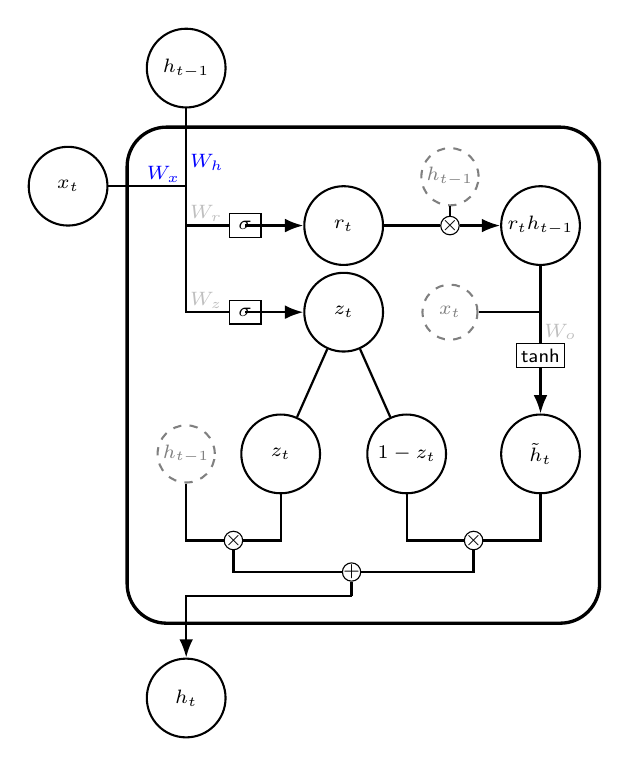
\begin{tikzpicture}[
    % GLOBAL CFG
    font=\sf \scriptsize,
    >=LaTeX,
    % Styles
    cell/.style={% For the main box
        rectangle, 
        rounded corners=5mm, 
        draw,
        very thick,
        },
    operator/.style={%For operators like +  and  x
        circle,
        draw,
        inner sep=-0.5pt,
        minimum height =.2cm,
        },
    function/.style={%For functions
        ellipse,
        draw,
        inner sep=1pt
        },
    ct/.style={% For external inputs and outputs
        circle,
        draw,
        line width = .75pt,
        minimum width=1cm,
        inner sep=1pt,
        },
    ctsmall/.style={
        circle,
        draw,
        line width = .75pt,
        minimum width=0.7cm,
        dashed,
        gray,
        inner sep=1pt,
        },
    gt/.style={% For internal inputs
        rectangle,
        draw,
        minimum width=4mm,
        minimum height=3mm,
        inner sep=1pt
        },
    mylabel/.style={% something new that I have learned
        font=\scriptsize\sffamily
        },
    ArrowC1/.style={% Arrows with rounded corners
        rounded corners=0cm,%.25cm,
        thick,
        },
    ArrowC2/.style={% Arrows with big rounded corners
        rounded corners=0cm,%.5cm,
        thick,
        },
    ]

%Start drawing the thing...    
    % Draw the cell: 
    \node [cell, minimum height =6.3cm, minimum width=6cm] at (0.75,0.1){} ;

    \newcommand{\step}{1.1}

    % Draw activation functions
    \node [gt] (sigma_f) at (-0.75,2) {$\sigma$};
    \node [gt] (sigma_i) at (-0.75,2-\step) {$\sigma$};

    

    
    \node[text width=0.3cm, text = blue] at (-1.85,2.65) {$W_x$};
    \node[text width=0.3cm, text = blue] at (-1.3,2.8) {$W_h$};
    
    
    \node[text width=0.3cm, text=lightgray] at (-1.3,2.15) {$W_r$};
    \node[text width=0.3cm, text=lightgray] at (-1.3,2.15-\step) {$W_z$};
    %\node[text width=0.3cm, text=lightgray] at (-1.3,2.15-2*\step) {$W_c$};
    \node[text width=0.3cm, text=lightgray] at (3.2,0.65) {$W_o$};
    
    % Draw Internal 
    \node[ct] (ft) at (0.5,2) {$r_t$};
    \node[ct] (it) at (0.5,2-\step) {$z_t$};

   % Draw multiplication and addition operators
    \node [operator] (mux_conveyor) at (1.85,2) {$\times$};
    
    \node [gt, minimum width=0.6cm] (add_conveyor) at (3,0.35) {tanh};
    
    \node [ctsmall] (hsmall) at (1.85,2+\step/2 + 0.07) {$h_{t-1}$};
    \node [ctsmall] (mux_i_and_c) at (1.85,2-\step) {$x_t$};
    \node [operator] (mux_end) at (0.6,2-4*\step) {$+$};
    
    \node [ctsmall] (hsmall_bottom) at (-1.5,-0.9) {$h_{t-1}$};
    \node[ct] (z_final) at (-0.3,-0.9) {$z_t$};
    \node[ct] (one_minus_z_final) at (1.3,-0.9) {$1-z_t$};
    \node[ct] (c2) at (3,-0.9) {$\tilde{h}_t$};


    % Draw External inputs? named as basis c,h,x
    %\node[ct, label={[mylabel]Cell}] (c_old) at (2.2,4) {$c_{t-1}$};
    \node[ct] (c_old) at (3,2) {$r_t h_{t-1}$};
    \node[ct] (h_old) at (-1.5,4) {$h_{t-1}$};
    \node[ct] (x) at (-3,2.5) {$x_t$};
    
    \node [operator] (times_left) at (-0.9,-2) {$\times$};
    \node [operator] (times_right) at (4.3/2,-2) {$\times$};
    
    

    % Draw External outputs? named as basis c2,h2,x2
    
    \node[ct] (h2) at (-1.5,-4) {$h_t$};
    
    

% Start connecting all.
    %Intersections and displacements are used. 
    % Drawing arrows    
    %\draw [->, ArrowC1] (c_old) -- (mux_conveyor) -- (add_conveyor) -- (c2);

    % Inputs
    \draw [->, ArrowC1] (h_old)++(0,-0.5) |- (sigma_f) |- (ft);
    \draw [->, ArrowC1] (h_old)++(0,-0.5) |- (sigma_i) |- (it);
    
    % f_t to the conveyor
    \draw [ArrowC1] (ft) -- (mux_conveyor);
    
    % i_t and hatC_t to the conveyor
    %draw [ArrowC1] (it) -| (mux_i_and_c)++(0,-0.5);
    \draw [ArrowC1] (mux_i_and_c) -| (add_conveyor);
    \draw [ArrowC1] (hsmall) -- (mux_conveyor);
    \draw [->, ArrowC1] (mux_conveyor) -- (c_old);
    
    \draw [->, ArrowC1] (c_old) -- (add_conveyor) -- (c2);
      
    



    \draw [ArrowC1] (it) -- (z_final);
    \draw [ArrowC1] (it) -- (one_minus_z_final);
    
    \draw [ArrowC1] (z_final) |- (times_left);
    \draw [ArrowC1] (hsmall_bottom) |- (times_left);
    
    \draw [ArrowC1] (one_minus_z_final) |- (times_right);
    \draw [ArrowC1] (c2) |- (times_right);

    %\node [ctsmall] (hsmall_bottom) at (-1.5,-0.9+0) {$h_{t-1}$};
    %\node[ct] (z_final) at (0,-0.9) {$z_t$};
    %\node[ct] (one_minus_z_final) at (1.5,-0.9) {$1-z_t$};
    %\node[ct] (c2) at (3,-0.9) {$\tilde{h}_t$};
    
    \draw [ArrowC1] (times_left) |- (mux_end);
    \draw [ArrowC1] (times_right) |- (mux_end);
    
    % end
    \draw [ArrowC1] (mux_end)++(0,-0.3) -- (mux_end);
    \draw [->, ArrowC1] (mux_end)++(0,-0.3) -| (h2);
    
    % begin
    \draw [ArrowC1] (x) -| (h_old)++(0,-0.3);
    

\end{tikzpicture}
\end{document}